\documentclass[12pt]{ctexart}

% 包含必要的包
\usepackage[utf8]{inputenc}
\usepackage{amsmath, amssymb}  % 数学符号包
\usepackage{graphicx}  % 插入图片的包
\usepackage{hyperref}  % 生成超链接
\usepackage{fancyhdr}  % 页眉页脚设置
\usepackage{geometry}  % 页面设置
\usepackage{titlesec}  % 用于自定义 section 的格式
\usepackage{float}
\usepackage{listings}
\usepackage{xcolor}

\geometry{a4paper, margin=1in}

\titleformat{\section}[hang]{\normalfont\Large\bfseries}{\thesection}{1em}{}

\lstset{
    language=Python,
    basicstyle=\ttfamily\small,
    keywordstyle=\color{blue},
    stringstyle=\color{red},
    commentstyle=\color{green!50!black},
    numbers=left,
    numberstyle=\tiny\color{gray},
    frame=single,
    breaklines=true,
    backgroundcolor=\color{gray!10},
    showstringspaces=false,
    % captionpos=b % 让代码标题出现在代码下方
}

% Header and footer
\setlength{\headheight}{14.49998pt}
\addtolength{\topmargin}{-2.49998pt}

\pagestyle{fancy}
\fancyhf{}
\fancyhead[L]{《统计信号处理》实验报告}
% \fancyhead[M]{清华大学}
\fancyhead[R]{刘昱杉 2024214103}
\fancyfoot[C]{\thepage}



\begin{document}

\begin{titlepage}
    \begin{center}
        % Insert logo
        
\includegraphics[width=5cm]{tsinghua_logo.png}\\[4cm]  % 插入图标并设置下方间距
        {\Huge 实验四:图像分类与恢复实验} \\[4cm]
        {\large 刘昱杉  \ \  2024214103}\\[6cm]
        {\normalsize \today}\\[1cm]
        \vfill
        \text{注:本实验报告为单人独立完成}\\
        \text{关于本实验报告对应的源码及实验环境,详见\texttt{code}目录下\texttt{readme}}

    \end{center}
\end{titlepage}

\section*{FashionMnist图像分类实验}

\subsection*{实验原理}

本实验旨在利用 MindSpore 框架构建前馈神经网络,对 Fashion-MNIST 数据集进行分类任务。

Fashion-MNIST 数据集是一个包含 10 个类别的图像数据集,每个类别包含 6000 张训练图像和 1000 张测试图像,图像大小为 $28 \times 28$ 像素。
数据集中的 10 个类别分别为:T-shirt/top, Trouser, Pullover, Dress, Coat, Sandal, Shirt, Sneaker, Bag, Ankle boot。

\subsection*{实验步骤}

首先对数据集下载并预处理,并标定每张图片的数据格式:{通道数,图像长,宽,标签}
\begin{figure}[H]
    \centering
    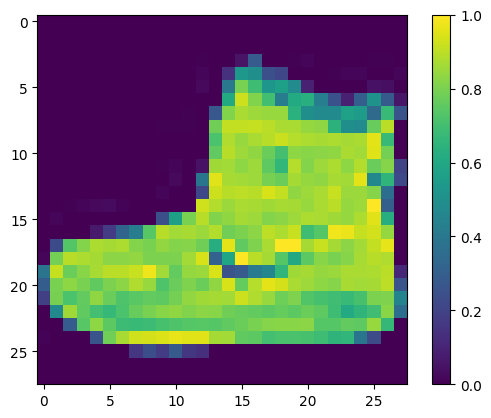
\includegraphics[width=0.7\textwidth]{image/1.png}
    \caption{FashionMnist数据可视化}
\end{figure}

然后构建前馈神经网络,包含两个隐藏层,每个隐藏层包含 128 个神经元,激活函数为 ReLU,输出层包含 10 个神经元,激活函数为 Softmax。
\newpage
\begin{lstlisting}[language=Python,caption={前馈神经网络模型}]
class Forward_fashion(nn.Cell):
    def __init__(self, num_classes=10, num_channel=1):
        super(Forward_fashion, self).__init__()
        self.conv1 = nn.Conv2d(num_channel, 6, 5, pad_mode='same')
        self.conv2 = nn.Conv2d(6, 16, 5, pad_mode='valid')
        self.relu = nn.ReLU()
        self.max_pool2d = nn.MaxPool2d(kernel_size=2, stride=2)
        self.flatten = nn.Flatten()
        self.fc1 = nn.Dense(16 * 5 * 5, 120, weight_init=Normal(0.02))
        self.fc2 = nn.Dense(120, 84, weight_init=Normal(0.02))
        self.fc3 = nn.Dense(84, num_classes, weight_init=Normal(0.02))
\end{lstlisting}

模型训练步骤如下:

\begin{itemize}
    \item 损失函数: Softmax 交叉熵计算多类别分类损失
    \item 优化器:Adam 优化器,自适应学习率调整
    \item 训练配置:使用回调函数记录损失值和保存检查点
\end{itemize}

\begin{lstlisting}[language=Python,caption={分类网络训练}]
net_loss = nn.SoftmaxCrossEntropyWithLogits(sparse=True, reduction="mean")
net_opt = nn.Adam(network.trainable_params(), learning_rate=cfg.lr)
model = Model(network, loss_fn=net_loss, optimizer=net_opt, metrics={"acc"})
loss_cb = LossMonitor(per_print_times=int(cfg.train_size / cfg.batch_size))
config_ck = CheckpointConfig(save_checkpoint_steps=cfg.save_checkpoint_steps,
                             keep_checkpoint_max=cfg.keep_checkpoint_max)
ckpoint_cb = ModelCheckpoint(prefix=cfg.output_prefix, directory=cfg.output_directory, config=config_ck)
print("============== Starting Training ==============")
model.train(cfg.epoch_size, ds_train, callbacks=[ckpoint_cb, loss_cb], dataset_sink_mode=False)
\end{lstlisting}

\section*{实验结果}

通过30轮训练,准确率不断提升,训练集准确率约95.7\%,随机选15张图片进行label预测,结果均正确。

\begin{figure}[H]
    \centering
    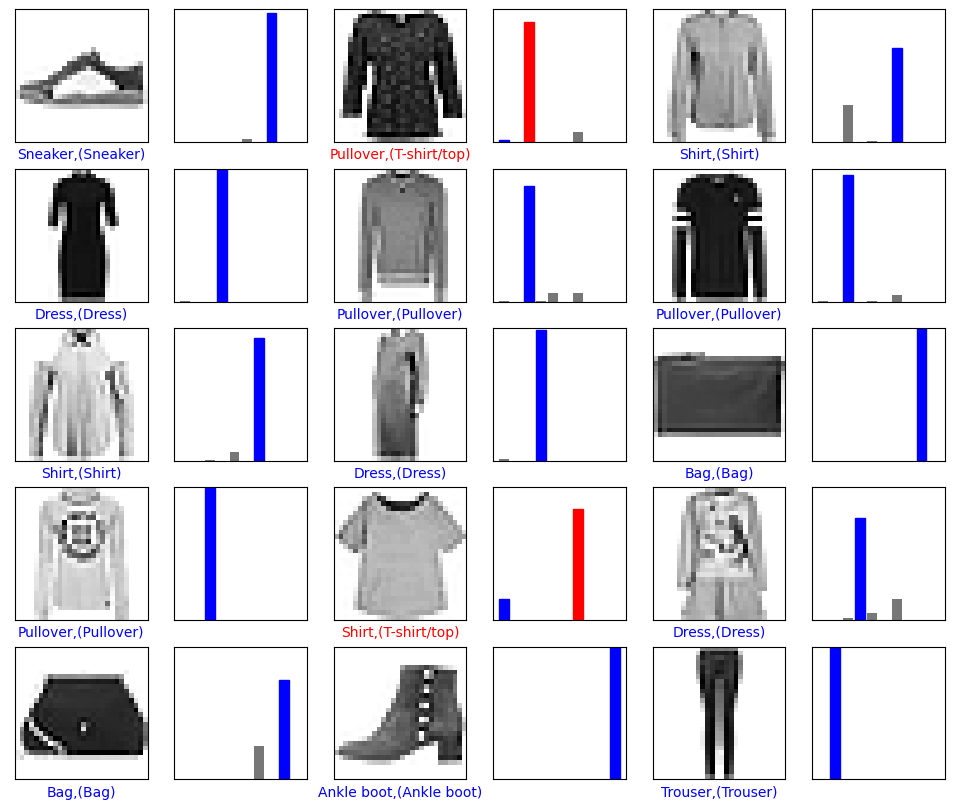
\includegraphics[width=0.7\textwidth]{image/2.png}
    \caption{FashionMnist分类结果}
\end{figure}

模型性能分析如下:
\begin{itemize}
    \item 优点:简单的前馈网络能够快速收敛,适用于中等规模数据集;网络参数适中,计算量较低。
    \item 缺点:未使用正则化或数据增强,可能存在一定程度的过拟合;网络结构较浅,对于更复杂的图像数据可能表现有限。
    \item 优化方向:增加正则化项,如Dropout、L2正则化;尝试更深的网络结构,如ResNet、VGG等。
\end{itemize}

\newpage

\section*{图像恢复实验}

\subsection*{实验原理}

图像作为重要的信息载体,在获取、传输、存储过程中常常受到噪声的影响。去除噪声的影响并恢复图像原本的信息,是计算机视觉中的一个重要研究问题。
本实验选择基于区域二元线性回归模型的图像去噪方法:

\begin{enumerate}
    \item \textbf{高斯噪声}:为图像添加噪声,模拟真实场景中的图像噪声。
    \item \textbf{区域回归建模}:对每个噪声像素,基于其邻域内未受污染的像素点进行回归建模,预测噪声点的像素值。
    \item \textbf{线性回归的图像恢复}:根据采用岭回归模型,对图像中的每个噪声像素进行像素值恢复。
\end{enumerate}

\subsection*{实验步骤}

首先生成高斯噪声图像,通过随机生成服从正态分布的噪声矩阵,并将噪声矩阵与原图像叠加,模拟真实场景中的图像噪声。

\begin{lstlisting}[language=Python,caption={生成高斯噪声}]
def add_noise(img, noise_ratio):
    #numpy.random.binomial(n,p,size=None)
    noise_img = np.random.binomial(1, 1 - noise_ratio, size=img.shape) 
    noise_img = np.multiply(noise_img,img)
    return noise_img
\end{lstlisting}
为原始图片添加了90\%的高斯噪声,得到如下图像对比:
\begin{figure}[H]
    \centering
    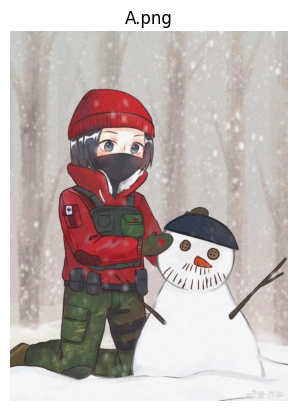
\includegraphics[width=0.4\textwidth]{image/3.png}
    \caption{初始图象}
\end{figure}

\begin{figure}[H]
    \centering
    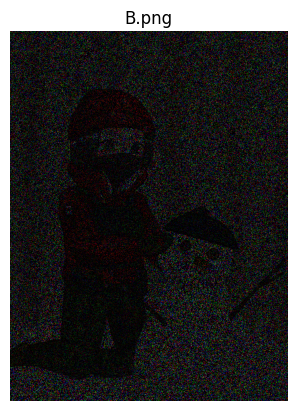
\includegraphics[width=0.4\textwidth]{image/4.png}
    \caption{高斯噪声图象}
\end{figure}

然后对噪声图像进行区域回归建模,对每个噪声像素点,利用其邻域内的未受污染的像素点进行线性回归建模,预测噪声点的像素值。
通过计算恢复程度来结束迭代,并计算最终恢复图像与初始图像的loss值。
\newpage
\begin{lstlisting}[language=Python,caption={复原图像函数}]
def restore(img, domain_length): 
    resImg = np.copy(img)
    noiseMask = np.array(img != 0, dtype='double')
    rows, cols, channel = img.shape
    count = 0
    for row in range(rows):
        for col in range(cols):
            for chan in range(channel):
                if noiseMask[row, col, chan] != 0.:
                    continue
                x_train = []
                y_train = []
                for i in range(row-domain_length, row+domain_length):
                    if i < 0 or i >= row:
                        continue
                    for j in range(col-domain_length, col+domain_length):
                        if j < 0 or j >= col:
                            continue
                        elif noiseMask[i, j, chan] == 0.:
                            continue
                        elif i == row and j == col:
                            continue
                        x_train.append([i, j])
                        y_train.append([img[i, j, chan]])  
                if x_train == []:
                    continue
                Regression = LinearRegression()   
                Regression.fit(x_train, y_train)  
                resImg[row, col, chan] = Regression.predict([[row, col]])
            count += 1
            if count % 5000 == 0:
                print("picture restored:" +
                        str(float(count)/rows/cols))       
    print("picture restore finish!")
    return resImg
\end{lstlisting}



\section*{实验结果}

通过区域回归建模,对高斯噪声图像进行像素值恢复,得到如下结果,同时loss从初始的1136.72降低为716.79。
由于人为加入噪声比例很大,恢复图像可以大致看出初始图像的全貌,可以认为恢复算法效果较好。

\begin{figure}[H]
    \centering
    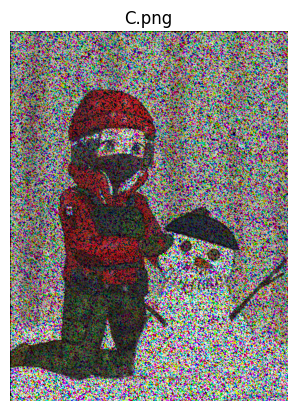
\includegraphics[width=0.4\textwidth]{image/5.png}
    \caption{恢复图像}
\end{figure}

\textbf{可能的改进}
\begin{itemize}
    \item 批量处理:对多个噪声点同时进行建模与预测,提升计算效率。
    \item 采用深度学习方法:使用卷积神经网络等深度学习方法,对图像进行去噪处理。
    \item 区域自适应:根据噪声点分布调整邻域大小,提高恢复效果。
\end{itemize}


\newpage
\begin{thebibliography}{99}

    \bibitem{Schonhoff2007}
    T.A. Schonhoff \& A.A. Giordano, \textit{Detection and Estimation: Theory and its Applications}. Pearson Education, Inc., 2007. (信号检测与估计——理论与应用,关欣等译,电子工业出版社,2012年).
    
    \bibitem{Srinath1996}
    M.D. Srinath, P.K. Rajasekaran \& R. Viswanathan, \textit{Introduction to Statistical Signal Processing with Applications}. Prentice Hall, 1996.  
    
    \bibitem{Kay1993}
    Steven M. Kay, \textit{Fundamentals of Statistical Signal Processing, Volume I: Estimation Theory} (©1993) \& \textit{Volume II: Detection Theory} (©1998). Pearson Education. (《统计信号处理基础:估计与检测理论(卷 I、卷 II合集)》,罗鹏飞等译,电子工业出版社,2023年).  
    
    \bibitem{Candy2016}
    James V. Candy, \textit{Bayesian Signal Processing: Classical, Modern, and Particle Filtering Methods} (2nd ed.). John Wiley \& Sons, Inc., 2016. (宗华等译,哈尔滨工业大学出版社,2023年).  
    
    \bibitem{VanTrees2013}
    Harry L. Van Trees, Kristine L. Bell, with Zhi Tian, \textit{Detection Estimation and Modulation Theory, Part I: Detection, Estimation, and Filtering Theory} (2nd ed.). John Wiley \& Sons, Inc., 2013.  
    
    \bibitem{ChatGPT2024}
    ChatGPT by OpenAI (2024). Personal communication and consultation for generating LaTeX formatting, experimental methodology, and model evaluation strategies. OpenAI, \url{https://www.openai.com}.  
    
\end{thebibliography}
    
    

\end{document}